\documentclass{beamer}

\graphicspath{{img/}}

\usepackage{appendixnumberbeamer}

\usepackage{datetime}
\newdate{defensedate}{06}{09}{2017}
\newdate{startdate}{15}{05}{2017}
\newdate{enddate}{04}{08}{2017}

\usepackage{minted}

\usetheme[sectionpage=progressbar,subsectionpage=progressbar,numbering=fraction,
          progressbar=foot]{metropolis}

\title{Automated Test Data Generation for Dynamically-Typed Programming Languages}
\subtitle{Supervisor: Shin Yoo\\COINSE Lab, KAIST, South-Korea\\\displaydate{startdate} -- \displaydate{enddate}}

\date{\displaydate{defensedate}}
\author{%
  Simon Bihel\hfill\url{simon.bihel@ens-rennes.fr} \\
}
\institute{%
  University of Rennes I \\
  \'Ecole Normale Sup\'erieure de Rennes
}

\begin{document}

\maketitle

\begin{frame}{Table of contents}
  \setbeamertemplate{section in toc}[sections numbered]
  \tableofcontents[hideallsubsections]
\end{frame}


% \section*{Introduction}

\section{Automated Test Data Generation}

\begin{frame}{Tests are important}
  Tests are essentials to avoid bugs.
  \begin{itemize}
    \item .
  \end{itemize}

  But writing them by hand is:
  \begin{itemize}
    \item time-consuming,
    \item error-prone.
  \end{itemize}
\end{frame}

\begin{frame}{Test Data Generation}
  Generate inputs to satisfy some metrics.

  Many criteria:
  \begin{itemize}
    \item code coverage,
    \item
  \end{itemize}
\end{frame}

\begin{frame}[fragile]{Pathwise tests}
  \begin{columns}
    \begin{column}{0.5\textwidth}
      \begin{minted}{c}
void test(char x,char y) {
  if (x=='x')
    printf(" ");
  else
    printf("  ");
  if (x==y)
    printf("Equal");
  else
    printf("Not Equal");
}
      \end{minted}
    \end{column}
    \begin{column}{0.5\textwidth}
      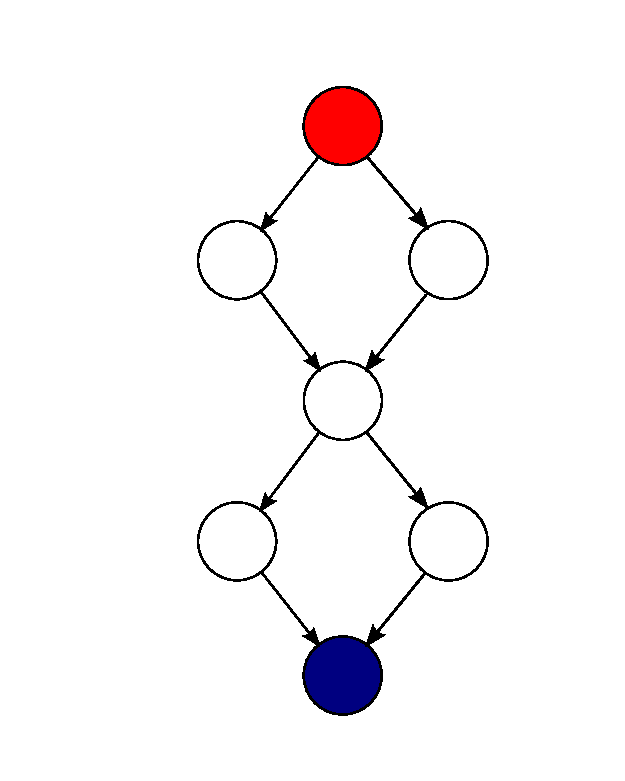
\includegraphics[height=\textheight]{Control_flow_graph}
    \end{column}
  \end{columns}
\end{frame}


\section{A Tool for Dynamically-Typed Languages}

\begin{frame}{Background}
  \begin{itemize}
    \item Started as a fork of CAVM (a tool for \texttt{C})
  \end{itemize}
\end{frame}

\begin{frame}{}
\end{frame}


\section{Challenges}

\begin{frame}{Dynamic types problems}
  \begin{itemize}
    \item Type errors
    \item Relations between parameters
    \item Working but unfit types
    \item Difficulty to reduce domain of possible types
  \end{itemize}
\end{frame}

\begin{frame}{Bigger picture problems}
  Dynamic languages usually have other paradigms

  \begin{itemize}
    \item Controlling the environment
    \item Understanding results
    \item Infinite search spaces
    \item Dynamic data structures
    \item Dynamic insertion of code
    \item Objects state
  \end{itemize}
\end{frame}


\section*{Conclusion}

\begin{frame}{Conclusion}
\end{frame}


\end{document}
